\documentclass{beamer}
%\documentclass[aspectratio=169]{beamer} %如果需要16:9
\usepackage{ctex}
\usepackage{times}
\usepackage{multicol}
\usepackage{multirow}
\usetheme{Warsaw}
%\usecolortheme{beaver}     % use white-grey colour style
%\beamersetaveragebackground{black!10}
% This is only inserted into the PDF information catalog. Can be left out.
\subject{presentation}
\keywords{example}
\useinnertheme{circles}%{rectangles}
\setbeamertemplate{itemize item}{$\circledast$}%{\checkmark}

%% ======================================================
%%     preamble
%% ======================================================
\title{基于IOT的多传感器火灾检测系统设计}
%\subtitle{Making Slides with Beamer}
%% for single author
\author{Luoo}
%\institute{物理系}

%% for multi-authors
%\author
%{J.~LaTeX\inst{1} \and M.~Beamer\inst{2}}

\institute
{
  \inst{1}
  物理系~西安理工大学
  \and
  \inst{2}
   applied physics\\
  Xi'an University of Technology
}
\date{\today}

\logo{
\includegraphics[height=0.09\textwidth]{./logo/xaut_logo}}


%% ======================================================
\begin{document}

%% ++++++++++++++++++++++++++++++++++++++++++++++++++++++
%% title page
%% ++++++++++++++++++++++++++++++++++++++++++++++++++++++
\begin{frame}
  \titlepage
\end{frame}

%% ++++++++++++++++++++++++++++++++++++++++++++++++++++++
%%     Table of Contents
%% ++++++++++++++++++++++++++++++++++++++++++++++++++++++
%\begin{frame}
    %\frametitle{Contents}
    %\tableofcontents
    %% 显示1-4section,不显示subsection
    %\tableofcontents[hidesubsections,sections={<1-4>}]
%\end{frame}

%% ++++++++++++++++++++++++++++++++++++++++++++++++++++++
%%     main part
%% ++++++++++++++++++++++++++++++++++++++++++++++++++++++
%\section{概述}
\begin{frame}
  \frametitle{概述}
  %\framesubtitle{关于\LaTeX{}}
  \begin{enumerate}
    \item<1-> 概述设计的系统的机构及原理
    \item<2-> 系统硬件设计与实现,深入解析各个传感器模块,图示连接电路与工作流程。
    \item<3-> 描述主程序流程,系统性能测试。
  \end{enumerate}
\end{frame}


%% ++++++++++++++++++++++++++++++++++++++++++++++++++++++
%%      正文
%% ++++++++++++++++++++++++++++++++++++++++++++++++++++++
%\section{系统硬件设计与实现 }
%\subsection{系统结构}
\begin{frame}
  \frametitle{系统结构及原理}
  \begin{block}{主控模块}
	\begin{itemize}
		\item Arduino Mega 2560(ATmega2560)
	\end{itemize}
\end{block}
\pause
  \begin{block}{传感器模块}
	\begin{itemize}
		\item DHT11温湿度传感器
        \item MQ-2型气敏传感器
	\end{itemize}
\end{block}
\pause
\begin{block}{通信模块}
	\begin{itemize}
		\item ZigBee无线组网模块
	\end{itemize}
\end{block}
\pause
\begin{block}{IOT}
	\begin{itemize}
		\item Raspberry Pi 开发板
	\end{itemize}
\end{block}
\end{frame}

%% ++++++++++++++++++++++++++++++++++++++++++++++++++++++
%%      Equation & Figures
%% ++++++++++++++++++++++++++++++++++++++++++++++++++++++
\begin{frame}
\frametitle{系统原理图}

\begin{figure}
\centering
   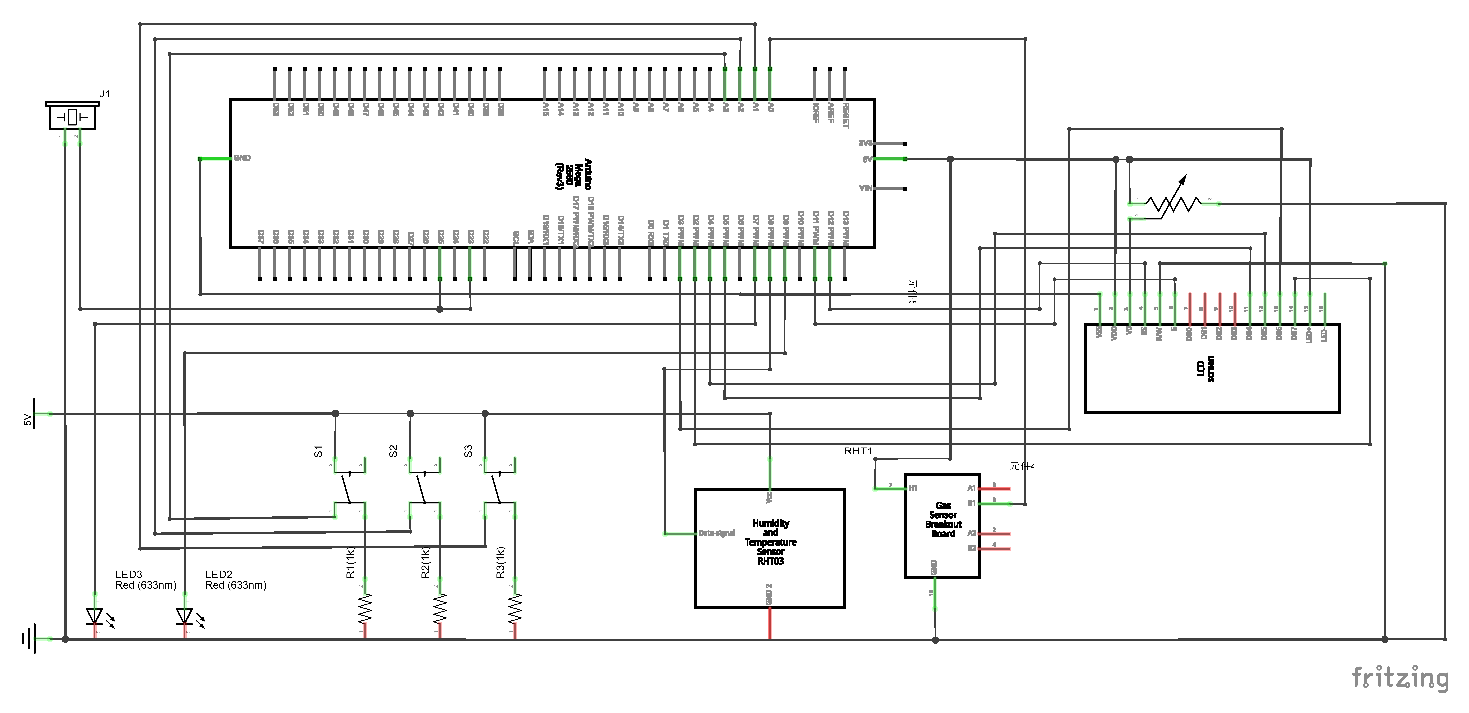
\includegraphics[height=6cm]{./img/U}
  \caption{主控模块电路图}
  \label{fig:visual}
\end{figure}

\end{frame}

\begin{frame}
\frametitle{实际装置图}
\begin{figure}
\centering
    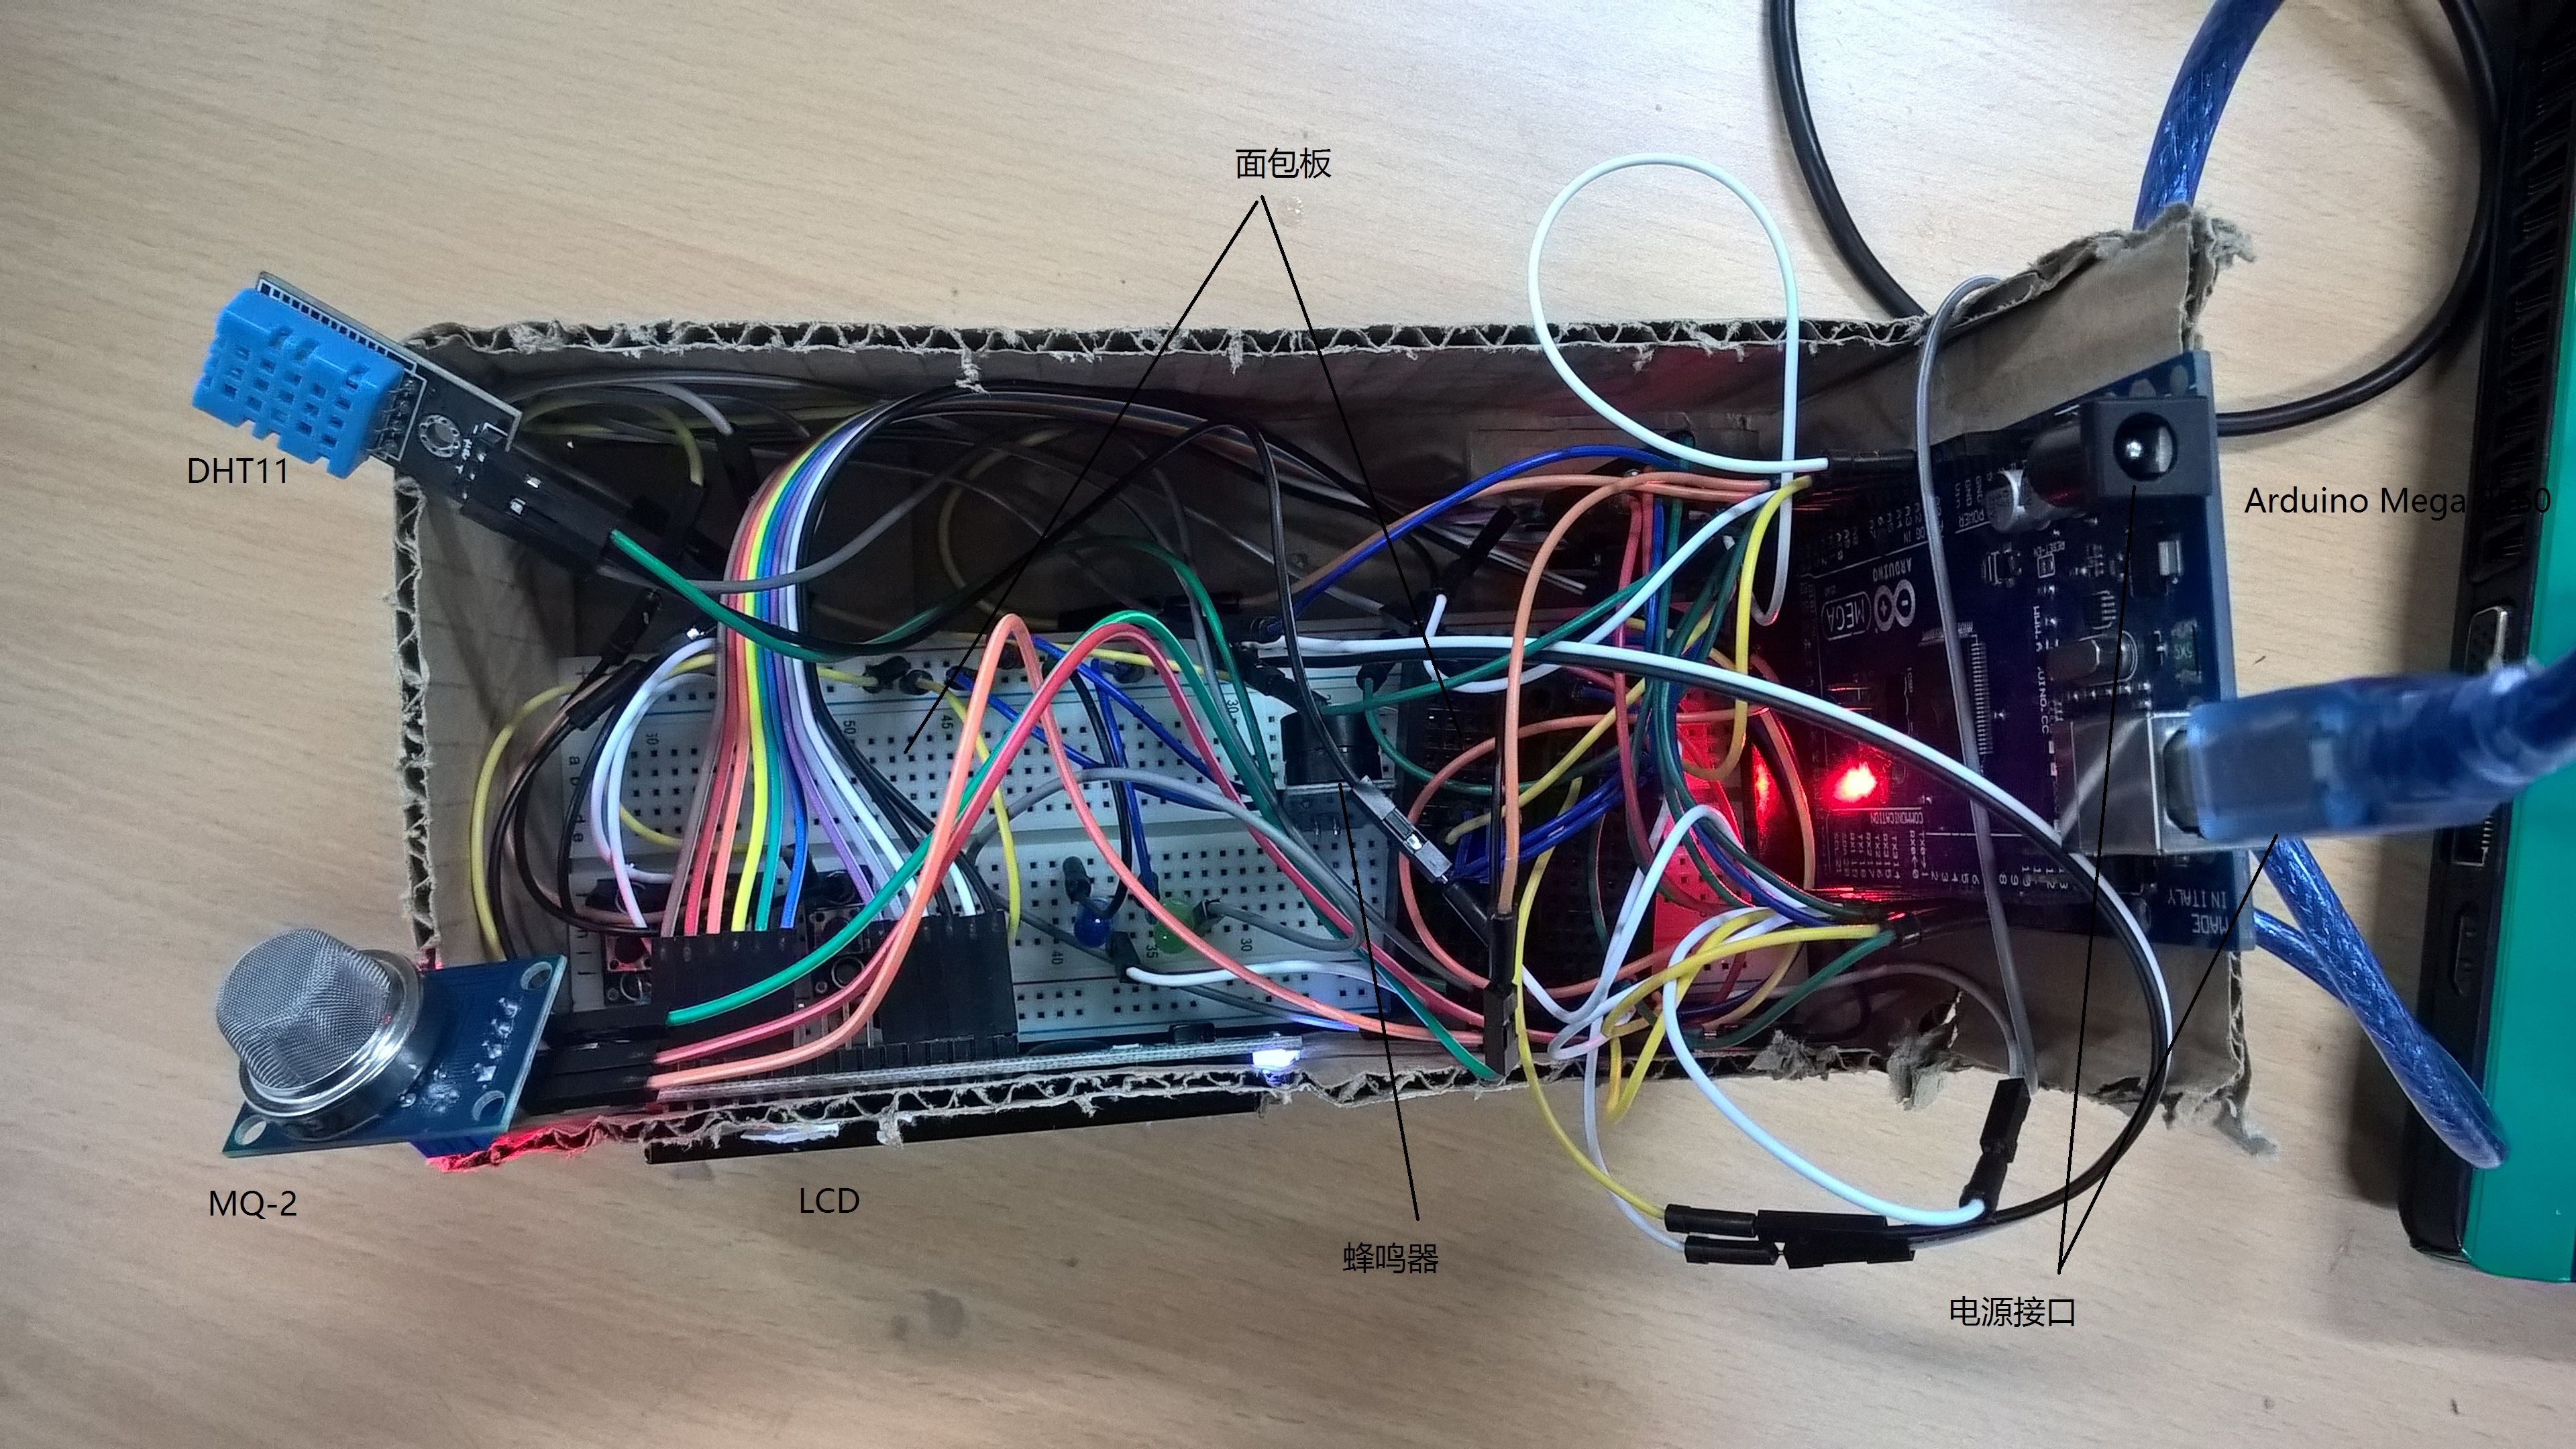
\includegraphics[height=6cm]{./img/wp}
\caption{实际装置图}
  \label{fig:visual}
\end{figure}
\end{frame}

%\subsection{传感器模块}
\begin{frame}
\frametitle{传感器模块}
\begin{columns}
\begin{column}{0.50\textwidth}
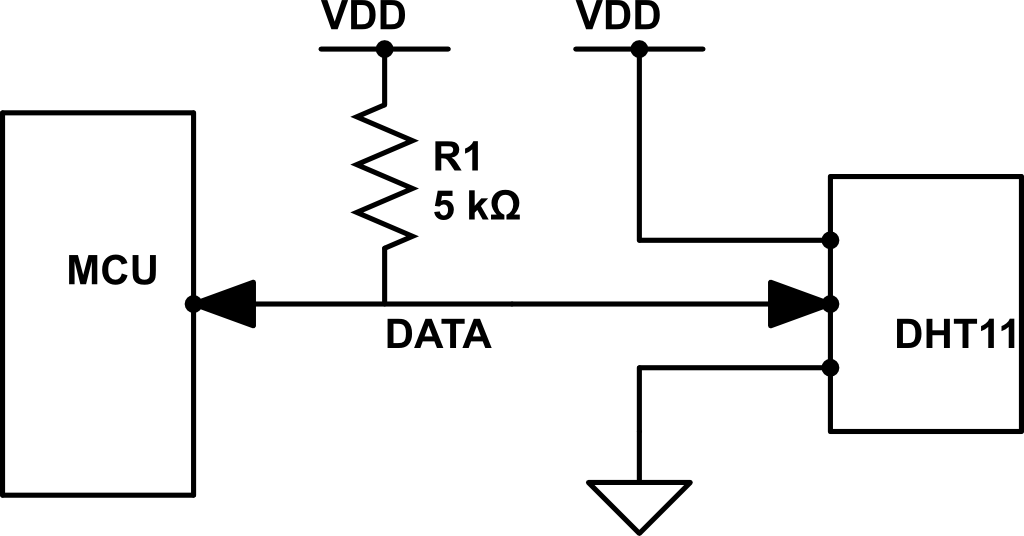
\includegraphics[width=\textwidth]{./img/dht11}
%\epsfig{figure=dht11,width=\textwidth}
\end{column}
\begin{column}{0.50\textwidth}
\begin{block}{DHT11}
\begin{enumerate}
\item 测量范围湿度20-90%,
温度$0-50℃$
\item 供电电压 3.3-5.5V DC
\item 全部校准,数字输出
\item 卓越的长期稳定性
\item 单总线串行接口的通信方式
\end{enumerate}
\end{block}
\end{column}
\end{columns}
\end{frame}

\begin{frame}
\frametitle{传感器}
\begin{columns}
\begin{column}{0.50\textwidth}
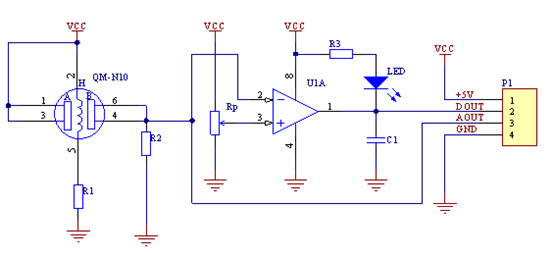
\includegraphics[width=\textwidth]{./img/M}
\end{column}
\begin{column}{0.50\textwidth}
\begin{block}{MQ-2烟雾传感器}
\begin{itemize}
\item 采用的气敏材
料是在清洁空气中电导率较低的二氧化锡(SnO 2 )。当它置于敏感气体环境
中时,其电导率随空气中敏感气体浓度的增大而增大。该传感器对于液化
气、丙烷和氢气的灵敏度非常高

\end{itemize}
\end{block}
\end{column}
\end{columns}
\end{frame}

%\subsection{网络联络}
\begin{frame}
\frametitle{数据联络}
\begin{columns}
\begin{column}{0.50\textwidth}
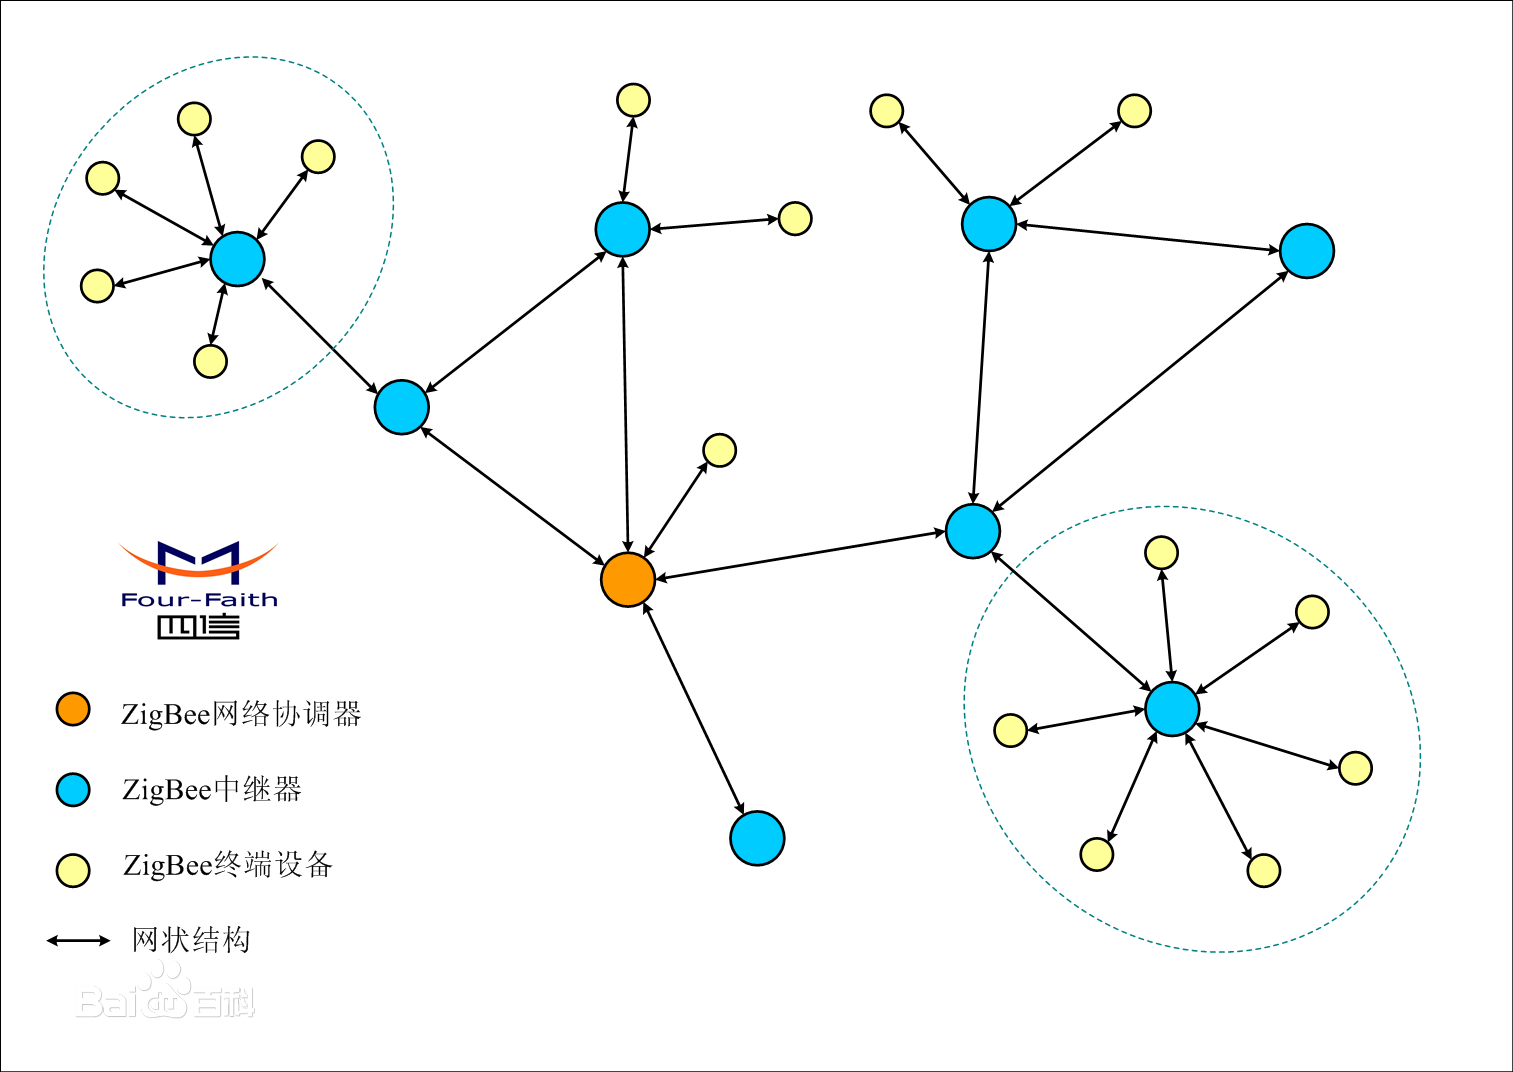
\includegraphics[width=\textwidth]{./img/z}
\end{column}
\begin{column}{0.50\textwidth}
\begin{block}{ZigBee无线通信技术}
\begin{enumerate}
\item 无线数据传输(2. 4 GHz 的无线信道)
\item 组网通信方式
\item 各传感器将采集的数据交由 MCU 进行数据处理,并给出局部判决结果
\end{enumerate}
\end{block}
\end{column}
\end{columns}
\end{frame}

\begin{frame}
\frametitle{IOT}
系统采用的结构是:Arduino+Raspberry Pi+Laravel+JSON+RESTful+Ajax+Python+HighCharts,Arduino与Raspberry Pi 通过串口通信的方式实现通信,相互传输所需要的数据,Raspberry Pi将资源传于互联网上对应的接口,接口可以在互联网上被访问。Laravel 框架构架于服务器之上,将Raspbery Pi获取过来的数据存储于MySQL数据,再以REST服务的方式共享数据,互联网上的其他设备便可以通过网络来访问这些设备。Ajax用于将后台的数据以不需要刷新的方式传递到网站前台,通过HighCharts框架显示给终端用户
\end{frame}
%\section{系统构建}
\begin{frame}
\frametitle{软件运作流程}
\begin{figure}
\centering
    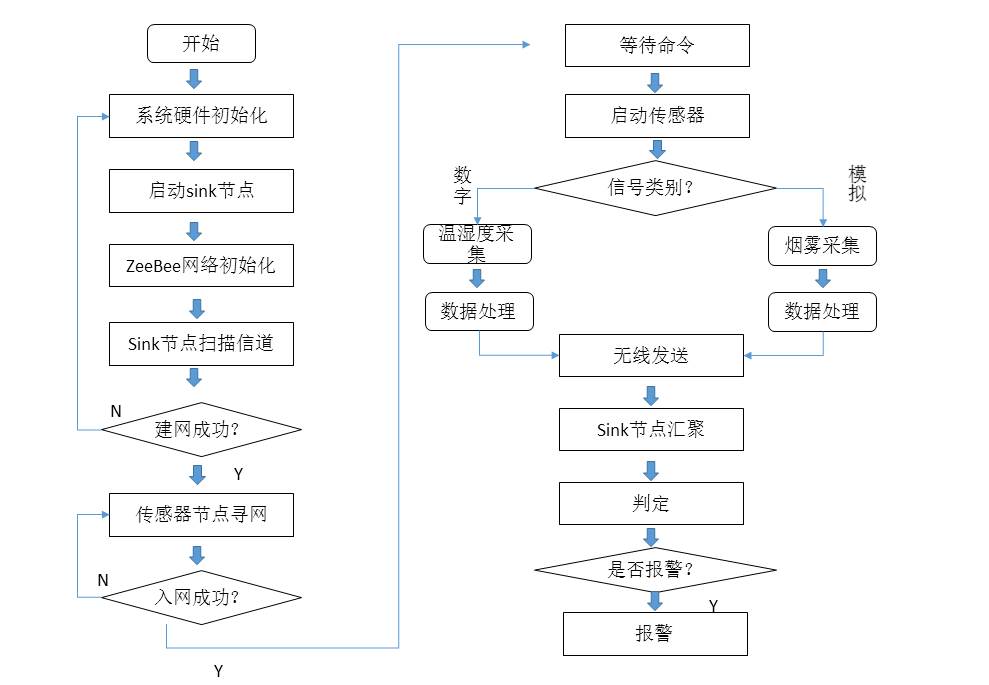
\includegraphics[height=6cm]{./img/all}
\end{figure}
\end{frame}

%\section{总结}
\begin{frame}
\frametitle{总结}
本火灾报警系统在满足基本的工作状态下,即在多传感器的阈值法进
行判定的基础上,加入 zigbee 无线技术,摒弃传统的总线方式,通过分布
式部署多传感器无线采集节点,克服了有线布线的弊端,解决了单传感器
检测准确性低等问题,有效提高了火灾预警系统的鲁棒性和报警的准确性。
同时加入以 REST 服务为核心,单片机、ARM 开发板为辅助的物联网系统,接入移动 PC 端,实现更多设备的连接,实现真正意义上的智能化火
灾报警系统。
\end{frame}
%% ++++++++++++++++++++++++++++++++++++++++++++++++++++++
%%      Last Page
%% ++++++++++++++++++++++++++++++++++++++++++++++++++++++
\begin{frame}
Thank You!

\end{frame}

%% ++++++++++++++++++++++++++++++++++++++++++++++++++++++
%%      Reference Page
%% ++++++++++++++++++++++++++++++++++++++++++++++++++++++
%\begin{frame}[allowframebreaks]{References}
  %\scriptsize
  %\bibliographystyle{apalike}
  %\bibliography{myRefs}
%\end{frame}

\end{document}
%% ======================================================
